% gjilguid2e.tex
% V2.0 released 1998 December 18
% V2.1 released 2003 October 7 -- Gregor Hutton, updated the web address for the style files.

\documentclass[mreferee]{gji}
\usepackage{timet}
\usepackage{amssymb}
\usepackage[cmex10]{amsmath}
\usepackage{mathtools, cuted}

\title[Geophys.\ J.\ Int.: \LaTeXe\ Guide for Authors]
	{Ensemble Source Encoding Full-waveform Inversion with Self-Adaptive Regularization}

%\author[B.L.N. Kennett]
%  {B.L.N. Kennett$^1$\thanks{Pacific Region Office, GJI} \\
%  $^1$ Research School of Earth Sciences, Australian National
%    University, Canberra ACT \emph{0200}, Australia
%  }

\author[C. He]
  {Conghui He$^{12}$, Yushu Chen$^2$, Bingwei Chen$^{12}$, Yunyue Li$^4$, Haohuan Fu$^{123}$, Guangwen Yang$^2$ \\
  $^1$ Ministry of Education Key Laboratory for Earth System Modeling, Department of Earth System Science, Tsinghua University, Beijing, China \\
  $^2$ Department of Computer Science and Technology, Tsinghua University, Beijing, China \\
  $^3$ Laboratory for Regional Oceanography and Numerical Modeling, Qingdao National Laboratory for Marine Science and Technology \\
  $^4$ Department of Civil and Environmental Engineering, National University of Singapore, Singapore
  }

\date{Received 1998 December 18; in original form 1998 November 22}
\pagerange{\pageref{firstpage}--\pageref{lastpage}}
\volume{200}
\pubyear{1998}

%\def\LaTeX{L\kern-.36em\raise.3ex\hbox{{\small A}}\kern-.15em
%    T\kern-.1667em\lower.7ex\hbox{E}\kern-.125emX}
%\def\LATeX{L\kern-.36em\raise.3ex\hbox{{\Large A}}\kern-.15em
%    T\kern-.1667em\lower.7ex\hbox{E}\kern-.125emX}
% Authors with AMS fonts and mssymb.tex can comment out the following
% line to get the correct symbol for Geophysical Journal International.
\let\leqslant=\leq

\newtheorem{theorem}{Theorem}[section]

\begin{document}

\label{firstpage}

\maketitle


\begin{summary}
We develop an ensemble source encoding full-waveform inversion method with self-adaptive regularization (EnFWI), which approximates the total inversion using the ensemble Kalman filter (EnKF) to alleviate the error caused by inaccurate initial model and data noise, and to further improve the computational efficiency. It refines an ensemble of velocity models simultaneously by iteratively incorporating the waveform observation, and approximates the nonlinear evolution of error covariance by the ensemble covariance. To overcome the problem in EnKF that the updating directions are confined in the low rank space spanned by the model samples which is lack of the representation ability in general, we apply the encoded simultaneous-source FWI (ESSFWI) to refine each model sample, so that the gradient directions along with perturbation are introduced to improve the representation ability of the low rank updating space. Along with the velocity, we use the EnKF scheme to adjust the anisotropic regularization factors in order to utilize the smoothing constrains in different directions to further reduce the model error. Experiments show that EnFWI achieves larger convergence range and better tolerance to data noise with less computational costs than the traditional FWI method.
\end{summary}

\begin{keywords}
Inverse theory; Controlled source seismology; Computational seismology; Wave propagation.
\end{keywords}

\section{Introduction}

Full-waveform inversion (FWI) is a promising data-fitting procedure which aims to extract quantitative information of the earth for high-resolution imaging from seismograms \cite{ta84}. However, FWI is a non-linear ill-posed problem which suffers from local convergence led by the initial model error and the lack of ultra-low frequency (ULF) data \cite{vi}. Data noise further deteriorates the imaging results.

Traditionally, the initial model is provided by some other methods such as traveltime tomography \cite{ls,pg,ss,pc,op,wo,wa} and migration velocity analysis \cite{al,sc,sb}. Other approaches to generate the initial model include first-arrival traveltime tomography \cite{ho}, stereotomography \cite{la}, Laplace-domain inversion and Laplace-Fourier-domain inversion \cite{sc08,sc09}, seismic envelope inversion \cite{wu,lw} and so on. These methods recover long-wavelength background structure to a certain extent, obtaining initial models with relatively low error. However, it is difficult to meet the demands of conventional gradient-based FWI that the initial model should produce synthetic data that are within a half-cycle, everywhere \cite{al}. Consequently, inversion methods with larger convergence domain are required.

Multiscale FWI methods \cite{bu,ra,vigh} are developed to reduce the initial model dependence by performing a cascade inversion starting from the lowest frequency available. The lowest frequency band (1.5-2.0 Hz) is crucial for these methods to recover the correct long-wavelength background-velocity structure. However, in most cases, the standard seismic records can go down only to approximately 5 Hz \cite{wu}. Not enough low frequency information is contained in the seismograms to avoid cycle skipping.

The conventional FWI is a simplification of the total inversion \cite{ta82}. Instead of minimizing the data misfit directly, the total inversion maximizes the posterior probability of the model parameters under certain initial model and seismograms as measurement. Comparing to FWI, the total inversion is less sensitive to initial model error and data noise \cite{ta84}. However, in the total inversion, the model and data covariance are required to generate the probability density function, leading to huge computation and memory costs, which make it actually impossible for high dimensional seismic inversion problems even with the state of art supercomputers.

The ensemble Kalman filter (EnKF) incorporates the initial model state and the observation using the same objective function as the total inversion \cite{ev94,ev03,ev09}. Instead of generating the covariance explicitly, it keeps an ensemble of model parameters, and uses the ensemble covariance to approximate the real covariance, providing an efficient mean to alleviate the computational costs. It has been applied in seismic inversion \cite{ji,qh}. However, in EnKF, the updating increment is confined in the low rank space spanned by the model samples. In high-dimensional problems, e.g., seismic explorations, where model parameters are several order of magnitudes larger than model samples, the low rank updating space is usually difficult to provide significant decreasing of the data misfit when the initial ensemble samples are generated by random perturbation. It is critical to adjust the model samples to improve the representation ability of the low rank space they spanned.

FWI with encoded simultaneous sources (ESSFWI) is an efficient tool to obtain a useful updating direction \cite{kr,be,ca}. It stacks the seismograms to reduce the number of forward modeling, which significantly reduces the computation, and uses different source codes in each updating step to suppress the noise resulting from crosstalk between the encoded sources. By the small fluctuations caused by source encoding, ESSFWI may even overcome small local minima \cite{ca}. However, ESSFWI is more sensitive to data noise \cite{kr} than FWI.

In this paper, we propose an ensemble source encoding full-waveform inversion method with self-adaptive regularization (EnFWI). In this method, we use EnKF to approximate the total inversion to enlarge the convergence domain and promote the resistance to data noise. ESSFWI is applied to refine the model samples to improve the representation for the low rank approximation. We also utilize the EnKF scheme to adjust the anisotropic regularization factor along with the velocity model, in order to utilize the smoothing constrains in different directions to further reduce the model error.

This paper is organized as follows. We firstly derive our EnFWI method. Then, we apply the method on the Marmousi model, to investigate the convergence range, the tolerance to data noise and the computational costs of EnFWI.


\section{Method}

In this section, we design the EnFWI scheme. We first apply the EnKF in seismic inversion problems to approximate the total inversion with low computational cost. Then we introduce ESSFWI to refine the model samples in order to improve the representation ability of the low rank updating space. We also use the EnKF scheme to adjust the anisotropic regularization factors in ESSFWI along with the model samples.

\subsection{Approximating the total inversion by EnKF}

In the seismic inversion problem, we need to obtain the underground model, from an initial model and the seismogram, which serves as an observation of the wave field. We here follow \cite{ev03} and apply the general EnFK theory to the seismic inversion problem.
For simplicity, we consider the acoustic FWI problem. The scalar wave equation is

\begin{equation}
m(x)\frac{\partial ^2{u}}{\partial{t^2}}(x,t)-\Delta u(x,t)=f,
\end{equation}
where $u$ is the pressure; the squared slowness $m=1/c^2$ is the model parameter to solve; $c$ is the wave velocity, and $f$ is the source term. The seismogram $d$ is the pressure $u$ recorded in seismic surveys. We define the measurement operator $H$ as $H_m=d_{cal}(m)$, where $d_{cal}(m)$ is the synthetic seismogram.

The total inversion and EnKF solve the inversion problem within the Bayesian framework. Assuming the posterior probability density function (PDF) to be Gaussian, in the $k$th updating step, by combining the prior knowledge of the initial model $(m_b)_k$, which is called the background field, and the observation $d_k$, the posterior PDF $p$ satisfies


\begin{equation}
%\resizebox{0.5\textwidth}{!}{$p \varpropto \exp\left ( -\left ( \left ( \left ( m_b \right )_k - m \right )^T B^{-1} \left ( \left ( m_b \right )_k -m\right ) +\left ( d_k-H_m \right )^TR_k^{-1}\left ( d_k-H_m \right )\right ) \right )$}
p \varpropto \exp\left ( -\left ( \left ( \left ( m_b \right )_k - m \right )^T B^{-1} \left ( \left ( m_b \right )_k -m\right ) +\left ( d_k-H_m \right )^TR_k^{-1}\left ( d_k-H_m \right )\right ) \right ),
\end{equation}
where $B$ is the covariance of $m_0$ and $R_k$ is the covariance of $d_k$.

To obtain the optimal model $m$ to maximize the posterior PDF $p$, we minimize the following objective function 
\begin{equation}
2S\left(m\right)=\left(\left(m_b\right)_k-m\right)^TB^{-1}\left(\left(m_b\right)_k-m\right)+\left(d_k-Hm\right)^T{R_k}^{-1}\left(d_k-Hm\right).
\end{equation}

By assigning the gradient of the objective function $S(m)$ to 0, we obtain
\begin{equation}
(m_a)_k=(m_b)_k+BH^T(HBH^T+R_k)^{-1}(d_k-H(m_b)_k),
\end{equation}
where $(m_a)_k$ is an optimal approximation of $m$ by combining the initial model $(m_b)_k$ and the observation $d_k$, and H is the tangent linear approximation of the measurement operator $H$.

According to eq. (4), the covariance of $(m_a)_k$, which is denoted by $P_k$, satisfies
\begin{equation}
P_k=B_k-B_k\mbox{H}^T(HB_k\mbox{H}^T+R_k)^{-1}\mbox{H}B_k.
\end{equation}

Eq. (4) and (5) form the analysis step of the extended Kalman filter (EKF), which is the nonlinear version of the Kalman filter (Kalman, 1960). However, huge computation is required. Denoting the dimension of slowness model $m$ and observation $d$ to be $N_m$ and $N_d$, the computation to generate $(\mbox{H}B_k\mbox{H}^T+R_k)^{-1}$ is $O(N_m^2N_d)$, the memory to store $B_k$ is $O(N_m^2)$, which are beyond the ability of modern computers for high dimension problems. Meanwhile, generating the tangent linear operator H also requires huge computation. Even worse is that the inverse operation may lead to numerical divergence.

EnKF solves these two problems by an ensemble approximation. We define the background model ensemble as $\Psi=(\psi_1^k,\psi_2^k,...,\psi_N^k)$, where $k$ is the number of the current updating step, $N$ is the number of model samples, $\psi_n^k, n\in\{1,2,...,N\}$ is a model sample. The initial model ensemble $\Psi_1$ is obtained by adding a spatial low frequency random perturbation field to the initial model $(m_b)_0$. We also generate an observation ensemble $D_k=(d_1^k,d_2^k,...,d_N^k)$ by adding Gaussian noise to the observation $d_k$. To save computation, we stack the sources and seismograms by different source codes in each updating step. Then, the model covariance $B$ and observation covariance $R$ at the $k$-th updating step are approximated as

\begin{equation}
\left\{
\begin{aligned}
& B_k=\Psi_k^{'}(\Psi_k^{'})^T/(N-1), \\
& R_k=D_k^{'}(D_k^{'})^T/(N-1),
\end{aligned}
\right.
\end{equation}
where $\Psi_k^{'}=\Psi_k(I-1_N)$ and $D_k^{'}=D_k(I-1_N)$.

By substituting the ensemble approximation eq. (6) into the updating rule eq. (4), we obtain

\begin{equation}
(\Psi_a)_k=\Psi_k+\Psi_k^{'}(\mbox{H}\Psi_k^{'})^T\left(\mbox{H}\Psi_k^{'}(\mbox{H}\Psi_k^{'})^T+D_k^{'}(D_k^{'})^T\right)^{-1}(D_k-H\Psi_k),
\end{equation}
where $(\Psi_a)_k$ is the analysis model ensemble, $\mbox{H}\Psi_k^{'}$ is computed as $H\Psi_k-\overline H\Psi_k$, with $\overline H\Psi_k$ the average of the synthetic records $H\Psi_k$. The tangent linear operator H need not to be generated explicitly. To reduce the computational costs of eq. (7) and eliminate the instability, by assuming $\mbox{H}\Psi_k^{'}$ and $D_k^{'}$ are independent, we obtain

\begin{equation}
\left(\mbox{H}\Psi_k^{'}(\mbox{H}(\Psi_k^{'})^T)+D_k^{'}(D_k^{'})^T\right)^{-1}\approx\left((\mbox{H}\Psi_k^{'}+D_k^{'})(\mbox{H}\Psi_k^{'}+D_k^{'})^T\right)^{-1}.
\end{equation}

By the SVD decomposition, we have

\begin{equation}
\mbox{H}\Psi_k^{'}+D_k^{'}=USV,
\end{equation}where U and V are orthogonal matrices, S is a diagonal matrix.

Then, the ensemble updating rule (7) turns to

\begin{equation}
(\Psi_a)_k=\Psi_k+\Psi_k^{'}(\mbox{H}\Psi_k^{'})^TU(SS^T)^{-1}U^T(D_k-H\Psi_k).
\end{equation}

For the real slowness model does not change, the analysis model ensemble $(\Psi_a)_k$ is used directly as the background model ensemble $\Psi_{k+1}$ in the next updating step.

In eq. (10), terms of the diagonal matrix $S$ with small absolute values correspond to updating directions which are not effectively represented by the ensemble. Consequently, we omit the small values and zeros of $S$ to enhance the stability. Then, at most $N$ columns of $U$ need to be generated. The dominate computational costs in eq. (10) is N forward modeling to generated $H\Psi_k$, and the memory cost is $O(N(N_m+N_d))$. In most applications, the sample number $N$ is chosen between 10 and 100. The computation is less than traditional FWI for the sources and seismograms are stacked. More memory is needed to store model samples if the method is run on one computing node; however, different model samples can be distributed on different nodes to make full use of the memory of a parallel computing cluster, while duplication of the model is also required on each node when traditional FWI is run in parallel on the same cluster. By the ensemble updating rule eq. (10), we apply the EnKF in the seismic inversion and approximate the total inversion with low computation and memory costs. However, in the eq. (10), the updating direction is confined in the space spanned by the background model ensemble $\Psi_k$. In general, if the initial background model ensemble $\Psi_1$ is generated by random perturbation, the low rank updating space cannot provide an effective updating direction which can significantly reduce the data misfit, especially in high dimensional problem where the model parameters are several order of magnitudes more than model samples. Improving the representation ability of the low rank updating space is crucial to provide clear imaging results.

\subsection{Refining the model samples using ESSFWI with self-adaptive regularization factors}

Bringing in effective updating directions may improve the representation ability of the low rank updating space spanned by the model samples. ESSFWI can provide such directions with low computational costs. It stacks the seismograms using different source codes in each updating step to save computation and suppresses the crosstalk noise. The anisotropic Tikhonov regularization term adds smoothing constraints with different weights in the horizontal and vertical direction. Take the 2D problem for example, the objective function of ESSFWI with anisotropic regularization term is

\begin{equation}
\left\{
\begin{aligned}
& S(m)=S_{data}(m)+S_{regu}(m) \\
& 2S_{data}(m)=||d-Hm||^2=\int_{0}^{T_{max}}\sum_{i=1}^{N_{rec}}||\hat u_o(r_{rec_i},t;f)-u_c(r_{rec_i},t;f)||^2dt \\
& 2S_{regu}(m)=\lambda_x||W_x||^2+\lambda_z||W_z||^2
\end{aligned}
\right.
\end{equation}
where $S_{data}(m)$ is the data misfit, $S_{regu}(m)$ is the anisotropic Tikhonov regularization term, $N_{rec}$ is the number of receivers, $r_{rec_i}$ is the position of the i-th receiver, $f$ is the stacked source using a random source code, $u_c(r_{rec_i},t;f)$ is the synthetic seismogram, $\hat u_o(r_{rec_i},t;f)$ is the stacked seismogram using the same source code, $\lambda_x$ and $\lambda_z$ are regularization factors. $W_x$ and $W_z$ indicate the discontinuity in the X and Z direction, as

\begin{equation}
\left\{
\begin{aligned}
& ||W_x||^2=\sum_{i=1}^{N_x-1}\sum_{j=1}^{N_z}\left(m(x_{i+1},z_j)-m(x_i,z_j)\right)^2 \\
& ||W_z||^2=\sum_{i=1}^{N_x}\sum_{j=1}^{N_z-1}\left(m(x_i,z_{j+1})-m(x_i,z_j)\right)^2
\end{aligned}
\right.
\end{equation}

Following Tarantola (1984), the gradient of the data misfit $S_{data}(m)$ can be computed as

\begin{equation}
G_{data}(m)=\int_{0}^{T_{max}}dt\sum_{i=1}^{N_{rec}}\frac{\partial}{\partial t^2}u^*(r,T_{max}-t;f)u(r,t;f)
\end{equation}
where $r$ is the position, $u^*(r,T_{max}-t;f)$ is the adjoint wavefield generated by propagate the data residual
\begin{equation}
\delta u(r_{rec_i},t;f)=\hat u_o(r_{rec_i},t;f)-u_c(r_{rec_i},t;f)
\end{equation}
backward in time.

In our realization of ESSFWI, the updating direction is obtained by the conjugate gradient (CG) method, and the step length is obtained by parabolic fitting. When it is used to refine the model samples in EnKF, we choose the negative gradient direction as the updating direction.

The regularization factors have a great influence on the inversion results. It is a challenging problem to find proper regularization factors. The EnKF scheme provides an efficient way to adjust the model samples and the regularization factors simultaneously. We define the new model ensemble combining the slowness model and the regularization factors as

\begin{equation}
\left\{
\begin{aligned}
& \Psi_k=\left(\psi_1^k,\psi_2^k,...,\psi_N^k\right), \\
& \psi_n^k=\left((\psi_n^k)^T,\lambda_x,\lambda_z\right)^T.
\end{aligned}
\right.
\end{equation}

We also expand the definitional domain of function $H$ to the new model sample $\psi_n^k$, as
\begin{equation}
H\psi_n^{k}=H\psi_n^{k}.
\end{equation}

We denote an updating step of the ESSFWI as

\begin{equation}
m_{k+1}=Lm_k.
\end{equation}

Then, we expand the definitional domain of function L to the new model sample as
\begin{equation}
L\Psi_n^k=L
\left(
\begin{aligned}
\psi_n^k \\
\lambda_x \\
\lambda_z
\end{aligned}
\right)
=
\left(
\begin{aligned}
& L\psi_n^k \\
& \lambda_x \\
& \lambda_z
\end{aligned}
\right).
\end{equation}

Following the ensemble updating rule eq. (7), we obtain the EnFWI as the analysis step
\begin{equation}
(\Psi_a)_k=\Psi_k+\Psi_k'(\mbox{H}\Psi_k')^T\left(\mbox{H}\Psi_k'(\mbox{H}\Psi_k')^T+D_k'(D_k')^T\right)^{-1}(D-H\Psi_k),
\end{equation}
and the model step
\begin{equation}
\Psi_{k+1}=L(\Psi_a)_k.
\end{equation}

In numerical experiments, we find that several updating steps of ESSFWI can be combined to accelerate the convergence, as

\begin{equation}
\Psi_{k+1}=L^{N_{iter}}(\Psi_a)_k,
\end{equation}
where $N^{iter}$ is typically chosen in [5,10].

\section{NUMERICAL RESULTS}
\subsection{Experiment Setup}
In order to examine the ability to tolerate inaccurate initial model and data noise, we applied our EnFWI method in Marmousi model to test results and compare them with FWI and ESSFWI.

The Marmousi model, shown in Figure \ref{fig:marmousi}, which is original 2301 grids in X-axis and 751 grids in Z-axis, is subsampled to 461 grids in X-axis and 151 grids in Z-axis, with the grid step of 20m. Equipped with Ricker wavelets with a peak frequency of 10Hz, 47 shots are placed at the interval of 200m each, at the depth of 120m for a period of 3s. 461 receivers are placed 20m each at the depth of 120m for recording the seismograms.

\begin{figure}
\center
\includegraphics[width=0.5\textwidth]{fig/marmvel.pdf}
\caption{True Marmousi model. The region highlighted is used for comparison with different methods.}
\label{fig:marmousi}
\end{figure}

A relatively large smoothing window size of 1200m in X-axis and 500m in Z-axis is applied on the true Marmousi model in the slowness domain, which is the initial model, shown in Figure \ref{fig:smoothed_model}.

\begin{figure}
\center
\includegraphics[width=0.5\textwidth]{fig/marmvel_smoothed.pdf}
\caption{Intial velocity model, smoothed by a 1200m x 500m window.}
\label{fig:smoothed_model}
\end{figure}

We make a forward modeling on the Marmousi model to acquire the seismograms, which are taken as inputs to three FWI methods, including conventional FWI, ESSFWI and EnFWI. We set the number of model samples in EnFWI to be 20, which can produce high resolution images at a low computational cost.

\subsection{Data Without Noise}

In the first experiment, seismograms are observed without data noise. The inversion results are shown in Figure \ref{fig:img_fwi}-\ref{fig:img_enfwi}. We can see that the velocity model inverted by FWI (Figure \ref{fig:img_fwi}) is in a low quality, which can just describe the very vague outline of the accurate model. Better than FWI, ESSFWI (Figure \ref{fig:img_esfwi}) can produce much clearer image especially in the middle and low-middle region, but ESSFWI is still trapped in local minima in some region. Compared to ESSFWI in the up-middle region of the image, EnFWI (Figure \ref{fig:img_enfwi}) can overcome these minima effectively and the layered structure is much smoother especially in the low-middle region.

\begin{figure}
\center
\includegraphics[width=0.5\textwidth]{fig/fwi.pdf}
\caption{Image inverted by conventional FWI method.}
\label{fig:img_fwi}
\end{figure}

\begin{figure}
\center
\includegraphics[width=0.5\textwidth]{fig/esfwi.pdf}
\caption{Image inverted by ESSFWI method.}
\label{fig:img_esfwi}
\end{figure}

\begin{figure}
\center
\includegraphics[width=0.5\textwidth]{fig/enfwi.pdf}
\caption{Image inverted by EnFWI. }
\label{fig:img_enfwi}
\end{figure}

Figure \ref{fig:l2norm} shows the variation of model misfit among three methods. Model misfit means the difference between the real model and the inverted model, which is measured by normalized L2 norm of slowness. Figure \ref{fig:l2norm} shows that the model misfit of FWI does not descend but those of ESSFWI and FWI are significantly improved. However, ESSFWI is trapped in local minima in the up-middle region.

\begin{figure}
\center
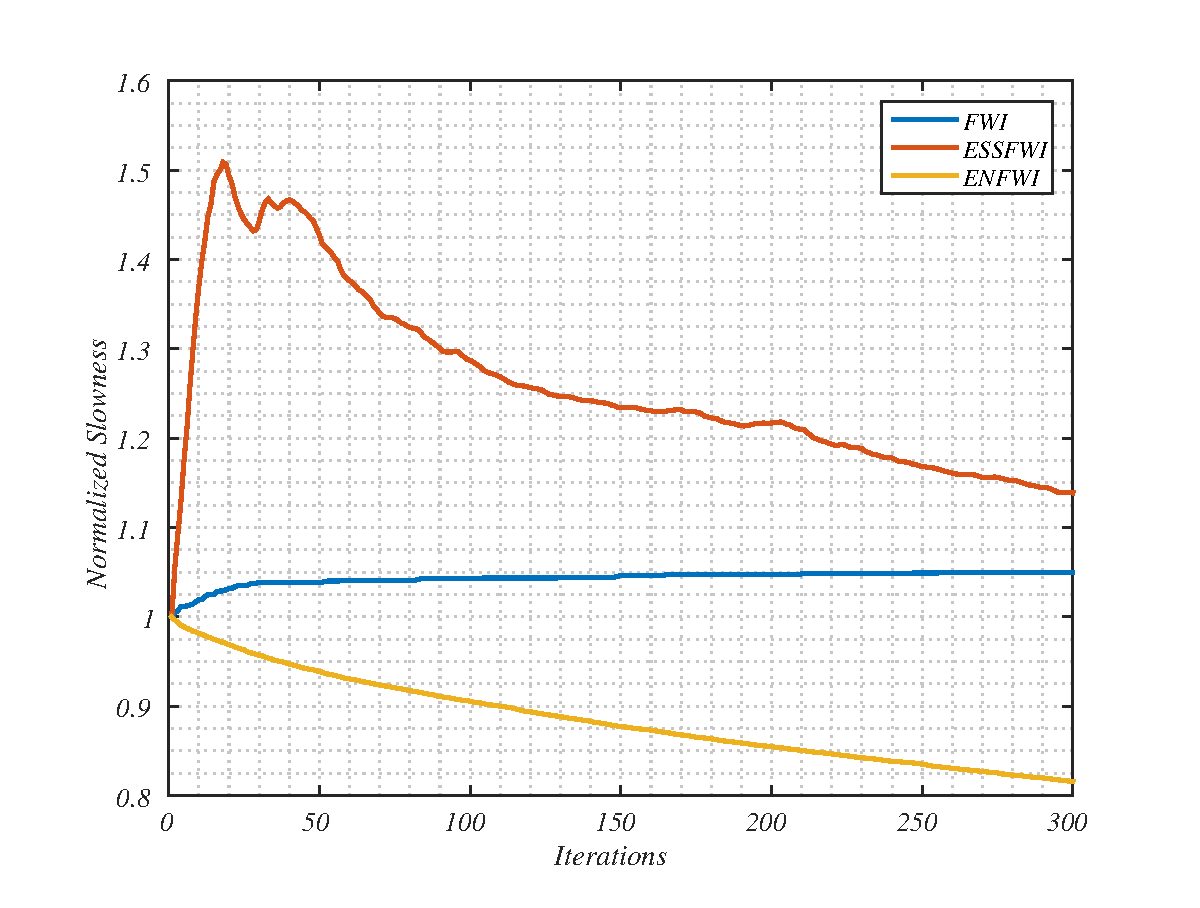
\includegraphics[width=0.5\textwidth]{fig/model_fit.eps}
\caption{Normalized L2-norm of the slowness error of FWI, ESSFWI and EnFWI without data noise.}
\label{fig:l2norm}
\end{figure}

\subsection{Data With Noise}
In the second experiment, we add white noise whose amplitude is 5\% of the maximum amplitude of the real seismograms to the data. Because most of the data is much smaller than their maximum, for this reason the noise is quite strong. Figure \ref{fig:img_fwi_noise}-\ref{fig:img_enfwi_noise}  show the inverted results. The imaging of FWI (Figure \ref{fig:img_fwi_noise}) is so vague and ESSFWI (Figure \ref{fig:img_esfwi_noise}) produce serious artifacts under the challenging strong noise. But our EnFWI (Figure \ref{fig:img_enfwi_noise}) can still reconstruct a good model.

\begin{figure}
\center
\includegraphics[width=0.5\textwidth]{fig/fwi-noise.pdf}
\caption{Velocity model inverted by FWI with data noise. The image is so vague.}
\label{fig:img_fwi_noise}
\end{figure}

\begin{figure}
\center
\includegraphics[width=0.5\textwidth]{fig/esfwi-noise.pdf}
\caption{Velocity inverted by ESSFWI with data noise. It falls into severe local minima.}
\label{fig:img_esfwi_noise}
\end{figure}

\begin{figure}
\center
\includegraphics[width=0.5\textwidth]{fig/enfwi-noise.pdf}
\caption{Image inverted by EnFWI. It can still get a better image under strong noise.}
\label{fig:img_enfwi_noise}
\end{figure}

\begin{figure}
\center
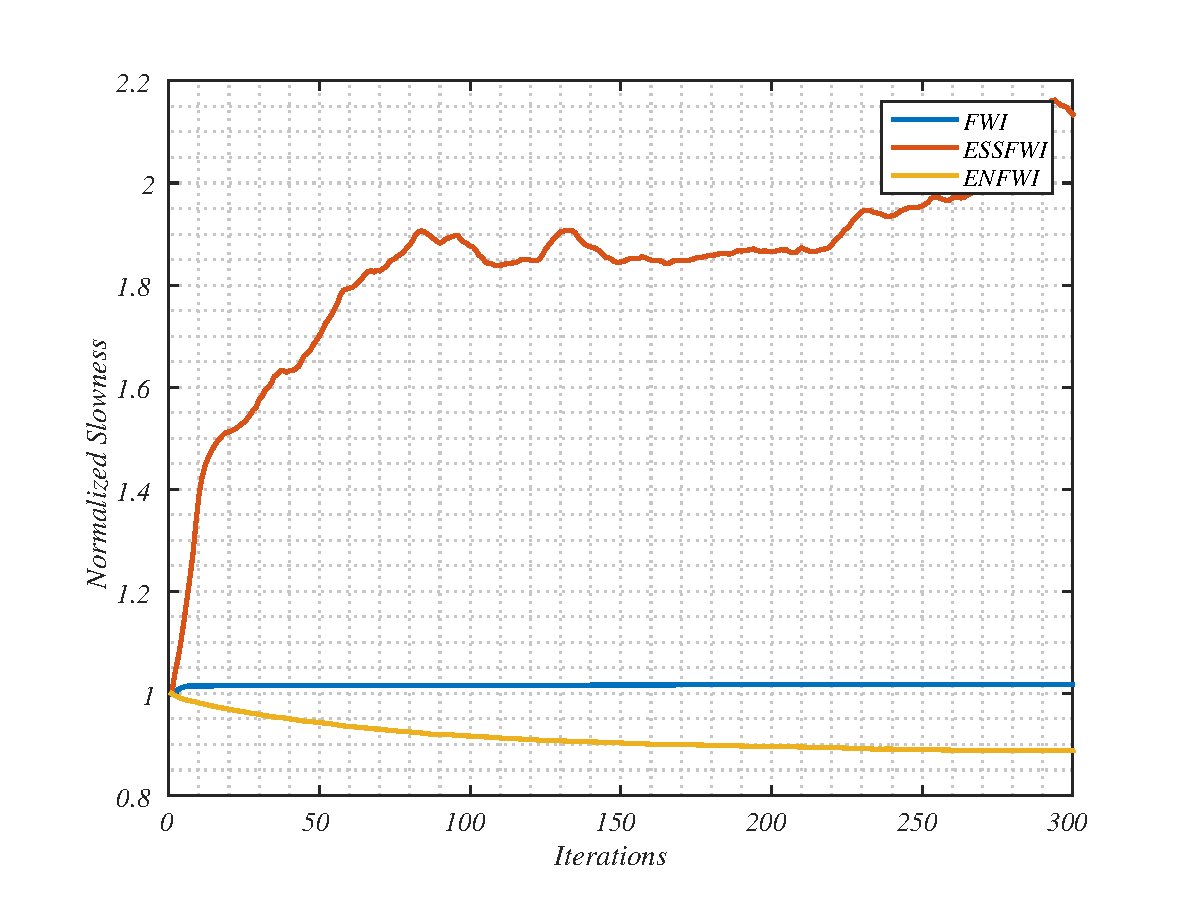
\includegraphics[width=0.5\textwidth]{fig/model_fit_noise.eps}
\caption{Normalized L2-norm of the slowness error of FWI, ESSFWI and EnFWI \textbf{with} data noise.}
\label{fig:l2norm_noise}
\end{figure}


In Figure \ref{fig:l2norm_noise}, under the strong noise, the model misfit of ESSFWI and FWI does not descend in a real sense, which means the inverted results are not ameliorated than the original model. The orange curve indicates that our EnFWI method can acquire much better convergence than ESSFWI and FWI.

\subsection{Performance}

Although the EnFWI method brings significant improvements on the representation of the inverted images, it also comes with additional computational cost. The computational cost is linearly increased with the number of samples in the model ensembles. The EssFWI is employed not only for improving the representation ability but also to reduce the computational cost of EnFWI, which makes EnFWI a practical imaging solution.

The normalized performance of FWI, EssFWI and EnFWI is shown in Figure \ref{fig:performance}. Compared with FWI, the computational cost of EssFWI is reduced by a factor roughly equal to the number of sources. On the other hand, the computational cost of EnFWI that employs EssFWI as the basic framework increases roughly linearly to the number of model samples. In our case where the number of sources is 40 and the number of model samples is 20, the EnFWI gains a speedup of 2x compared with FWI. Note that in a typical 3D case where the number of sources ranges from thousands to tens of thousands, the EnFWI method can gain a more significant speedup.

\begin{figure}
\center
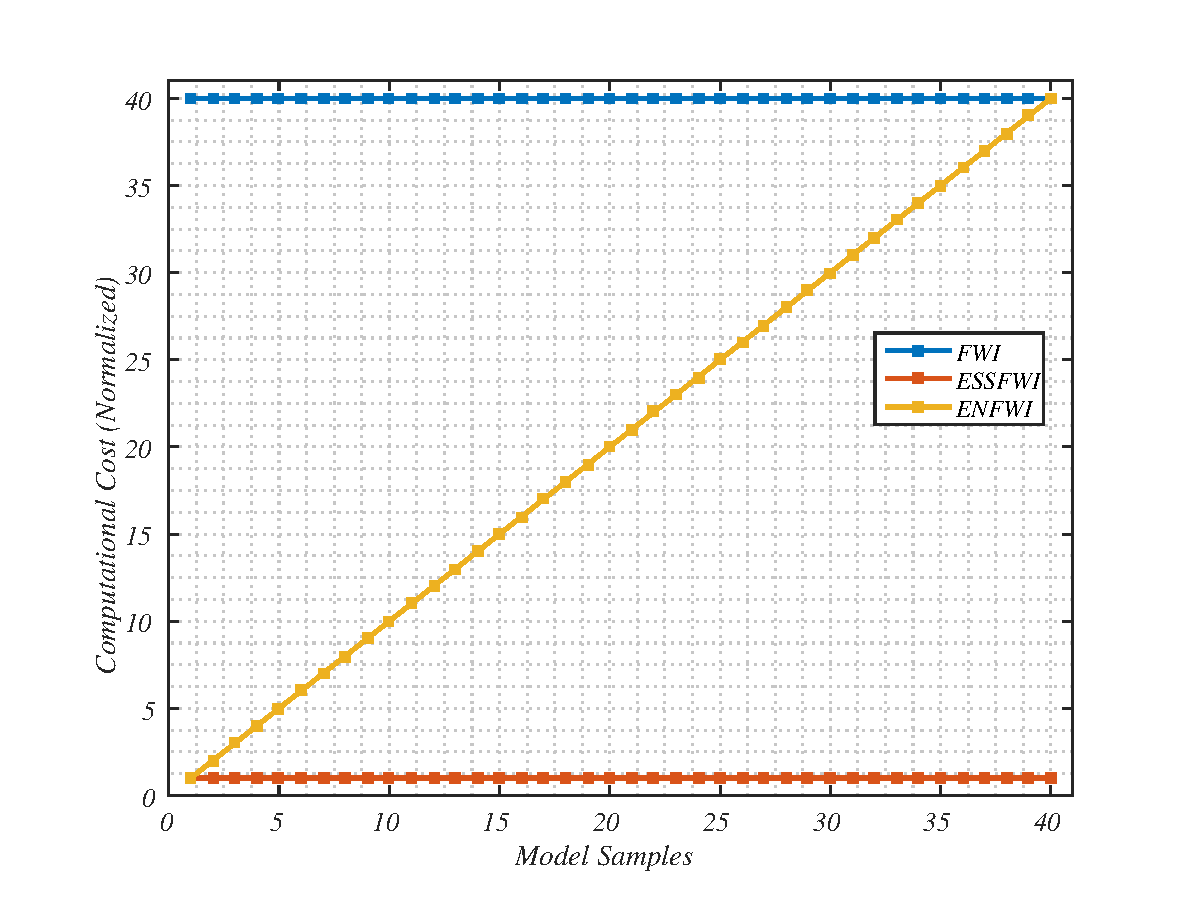
\includegraphics[width=0.5\textwidth]{fig/performance.eps}
\caption{The computational cost of FWI, EssFWI and EnFWI}
\label{fig:performance}
\end{figure}

\section{CONCLUSIONS}

We present an EnFWI method with self-adaptive regularization. It approximates the nonlinear evolution of the model covariance in the total inversion with an ensemble covariance to suppress the initial model error and data noise while keeping the computation within a realistic level. ESSFWI is also applied to improve the representation and performance. Anisotropic regularization with factors updated automatically in EnKF analysis steps is applied to decrease the artifacts utilizing the layered smooth constraints. Numerical experiments show that the proposed method not only has larger convergence range and better tolerance to data noise but also is more efficient than traditional FWI method.


\begin{acknowledgments}
A number of colleagues have helped with suggestions for the improvement of this material and I would particularly like to thank xxxxxxxxxxxxxxx. Dr. Yunyue Elita Li acknowledges the Singapore EDB Petroleum Engineering Professorship and Singapore Ministry of Education Tier-1 Grant R-302-000-182-114 for financial support.
\end{acknowledgments}

\begin{thebibliography}{}
\bibitem[\protect\citename{Al-Yahya }1989]{al} Al-Yahya, K., 1989. Velocity analysis by iterative profile migration, \textit{Geophysics}, \textbf{54}, 718-729.
  \bibitem[\protect\citename{Alkhalifah \& Choi }2014]{al} Alkhalifah, T. \& Choi, Y., 2014. From tomography to full-waveform inversion with a single objective function, \textit{Geophysics}, \textbf{79}, R55-R61.
  \bibitem[\protect\citename{Ben-Hadj-Ali et al. }2011]{be} Ben-Hadj-Ali, H., Operto, S. \& Virieux, J., 2011. An efficient frequency-domain full waveform inversion method using simultaneous encoded sources, \textit{Geophysics}, \textbf{76}, R109-R124.
\bibitem[\protect\citename{Bunks et al. }1995]{bu} Bunks, C., F.M. Saleck, S. Zaleski, and G. Chavent, 1995. Multiscale seismic waveform inversion,  \textit{Geophysics}, \textbf{60}, 1457-1473.
  \bibitem[\protect\citename{Castellanos et al. }2015]{ca}  Castellanos, C., Metivier, L., Operto, S., Brossier, R. \& Virieux, J., 2015. Fast full waveform inversion with source encoding and second-order optimization methods, \textit{Geophysical Journal International}, \textbf{200}, 720-744.
  \bibitem[\protect\citename{Evensen }1994]{ev94}  Evensen, G., 1994. Sequential data assimilation with a nonlinear quasi-geostrophic model using Monte Carlo methods to forecast error statistics, \textit{Journal of Geophysical Research: Oceans}, \textbf{99}, 10143-10162.
  \bibitem[\protect\citename{Evensen }2003]{ev03} Evensen, G., 2003. The ensemble Kalman Filter: theoretical formulation and practical implementation, \textit{Ocean Dynamics}, \textbf{53}, 343-367.
  \bibitem[\protect\citename{Evensen }2009]{ev09} Evensen, G., 2009. The ensemble Kalman filter for combined state and parameter estimation, \textit{Control Systems, IEEE}, \textbf{29}, 83-104.
\bibitem[\protect\citename{Hole }1992]{ho} Hole, J. A., 1992. Nonlinear high-resolution three-dimensional seismic travel time tomography, \textit{Journal of Geophysical Research}, \textbf{97}, 6553-6562.
\bibitem[\protect\citename{Jin et al. }2008]{ji} Jin, L., Sen, M.K. \& Stoffa, P.L., 2008. One-dimensional prestack seismic waveform inversion using ensemble Kalman filter, \textit{SEG Annu. Meet. Las Vegas, USA}.
  \bibitem[\protect\citename{Krebs et al. }2009]{kr} Krebs, J.R., Anderson, J.E., Hinkley, D., Neelamani, R., Lee, S., Baumstein, A. \& Lacasse, M.-D., 2009. Fast full-wavefield seismic inversion using encoded sources, \textit{Geophysics}, \textbf{74}, WCC177-WCC188.
  \bibitem[\protect\citename{Lambar$\acute{\textrm{e}}$ }2008]{la} Lambar$\acute{\textrm{e}}$, G., 2008. Stereotomography, \textit{Geophysics}, \textbf{73}, no. 5, VE25-VE34.
  \bibitem[\protect\citename{Luo \& Schuster }1991]{ls} Luo, Y. \& Schuster, G.T., 1991. Wave-equation traveltime inversion, \textit{Geophysics}, \textbf{56}, 645-653.
\bibitem[\protect\citename{Luo \& Wu }2015]{lw} Luo, J. and Wu, R.-S., 2015. Seismic envelope inversion: reduction of local minima and noise resistance, \textit{Geophysical Prospecting}, \textbf{63}, 597-614.
\bibitem[\protect\citename{Operto et al. }2004]{op} Operto, S., C. Ravaut, L. Improta, J. Virieux, A. Herrero, \& P. Dellaversana, 2004. Quantitative imaging of complex structures from dense wide aperture seismic data by multiscale traveltime and waveform inversions: A case study, \textit{Geophysical Prospecting}, \textbf{52}, 625-651.
\bibitem[\protect\citename{Pratt \& Goulty }1991]{pg} Pratt, R. G., \& N. R. Goulty, 1991. Combining wave-equation imaging with traveltime tomography to form high-resolution images from crosshole data, \textit{Geophysics}, \textbf{56}, 208-224.
\bibitem[\protect\citename{Priolo \& Chiaruttini }2003]{pc} Priolo, E., \& C. Chiaruttini, 2003. Analytical and numerical analysis of tomographic resolution with band-limited signals, \textit{Geophysics}, \textbf{68}, 600-613.
\bibitem[\protect\citename{Quan \& Harris }2008]{qh} Quan, Y. \& Harris, J.M., 2008. Stochastic seismic inversion using both waveformand traveltime data and its application to time-lapse monitoring, \textit{SEG Annu. Meet. Las Vegas, USA}.
\bibitem[\protect\citename{Ravaut et al. }2004]{ra} Ravaut, C., S. Operto, L. Improta, J. Virieux, A. Herrero, and P. Dell' Aversana, 2004. Multiscale imaging of complex structures from multifold wide-aperture seismic data by frequency-domain full-waveform tomography: Application to a thrust belt, \textit{Geophysical Journal International}, \textbf{159}, 1032-1056.
\bibitem[\protect\citename{Sava \& Biondi }2004]{sb} Sava, P., and B. Biondi, 2004. Wave-equation migration velocity analysis--Part I: Theory, \textit{Geophysical Prospecting}, \textbf{52}, 593-606.
\bibitem[\protect\citename{Shipp \& Singh }2002]{ss} Shipp, R. M., \& S. C. Singh, 2002. Two-dimensional full wavefield inversion of wide-aperture marine seismic streamer data, \textit{Geophysical Journal International}, \textbf{151}, 325-344.
\bibitem[\protect\citename{Shin \& Cha }2008]{sc08} Shin, C., and Y. H. Cha, 2008. Waveform inversion in the Laplace domain, \textit{Geophysical Journal International}, \textbf{173}, 922-931.
\bibitem[\protect\citename{Shin \& Cha }2009]{sc09} Shin, C., and Y. H. Cha, 2009. Waveform inversion in the Laplace-Fourier domain, \textit{Geophysical Journal International}, \textbf{177}, 1067-1079.
\bibitem[\protect\citename{Symes \& Carazzone }1991]{sc} Symes, W., and J. J. Carazzone, 1991. Velocity inversion by differential semblance optimization, \textit{Geophysics}, \textbf{56}, 654-663.
  \bibitem[\protect\citename{Tarantola }1984]{ta84} Tarantola, A., 1984. Inversion of seismic reflection data in the acoustic approximation, \textit{Geophysics}, \textbf{49}, 1259-1266.
\bibitem[\protect\citename{Tarantola \& Valette }1982]{ta82} Tarantola, A. \& Valette, B., 1982. Generalized nonlinear inverse problems solved using the least squares criterion, \textit{Rev Geophys}, \textbf{20}, 219-232.
\bibitem[\protect\citename{Vigh \emph{et al.} }2011]{vigh} Vigh, D., J. Kapoor, N. Moldoveanu, and H. Li, 2011. Breakthrough acquisition and technologies for subsalt imaging, \textit{Geophysics}, \textbf{76}, no. 5, WB41-WB51.
  \bibitem[\protect\citename{Virieux \& Operto }2009]{vi}  Virieux, J. \& Operto, S., 2009. An overview of full-waveform inversion in exploration geophysics, \textit{Geophysics}, \textbf{74}, WCC1-WCC26.
\bibitem[\protect\citename{Wang et al. }2014]{wa} Wang, H., S. C. Singh, and H. Calandra, 2014. Integrated inversion using combined wave-equation tomography and full waveform inversion, \textit{Geophysical Journal International}, \textbf{198}, 430-446.
\bibitem[\protect\citename{Woodward et al. }2008]{wo} Woodward, M.J., Nichols, D., Zdraveva, O., Whitfield, P. \& Johns, T., 2008. A decade of tomography, \textit{GEOPHYSICS}, \textbf{73}, VE5-VE11.
\bibitem[\protect\citename{Wu et al. }2014]{wu} Wu, R.-S., Luo, J. \& Wu, B., 2014. Seismic envelope inversion and modulation signal model, \textit{Geophysics}, \textbf{79}, WA13-WA24.

%Kalman, E., 1960. A new approach to linear filtering and prediction problems. Journal of Fluids Engineering, 82(1), 35-45.
\end{thebibliography}



\end{document}
